\documentclass[runningheads, 10pt]{article}

\usepackage[latin1]{inputenc}
\usepackage[T1]{fontenc}
%\usepackage{lmodern} % lmodern times fourier
%\usepackage{}
\usepackage[margin=2cm]{geometry}
\usepackage{lscape,enumitem,microtype}
\tolerance=1 \emergencystretch=\maxdimen \hyphenpenalty=10000 \hbadness=10000
\setlength{\parindent}{0em} \setlength{\parskip}{1em}

\usepackage{physics,siunitx}
\sisetup{per-mode=symbol-or-fraction, bracket-unit-denominator=false}
\usepackage{amsmath,amsfonts,amssymb,amsthm,bm} % bm for italic-bold in math
\usepackage{booktabs,multirow,multicol,makecell,array,longtable}
\usepackage{graphicx}
\usepackage{caption}
\usepackage[caption=false]{subfig}%{subcaption}

%\usepackage{algorithm}
%\usepackage{algorithmic}
%\algsetup{linenosize=\small,linenodelimiter=.}
%\DeclareCaptionFormat{algor}{%
%	\hrulefill\par\offinterlineskip\vskip1pt%
%	\textbf{#1#2}#3\offinterlineskip\hrulefill}
%\DeclareCaptionStyle{algori}{singlelinecheck=off,format=algor,labelsep=space}
%\captionsetup[algorithm]{style=algori}
\newcommand{\INPUT}{\item[\textbf{Input:}]}
\newcommand{\OUTPUT}{\item[\textbf{Output:}]}
\usepackage[ruled,linesnumbered,vlined]{algorithm2e} % [ruled,vlined]

\usepackage{hyperref}
\usepackage[nameinlink]{cleveref} %[noabbrev,nameinlink]




\newcommand{\diag}{\text{diag}}
\newcommand{\tpose}[1][T]{^\text{#1}}
\newcommand{\bpose}[1]{_\text{#1}}
\newcommand{\Bmtrx}[1]{\begin{bmatrix}#1\end{bmatrix}}
\newcommand{\bmtrx}[1]{\left[ #1 \right]}
\newcommand{\vex}[1]{\left[ #1 \times \right]}
\newcommand{\multiline}[1]{\begin{itemize}[leftmargin=.75em,topsep=-1em,itemsep=0em]#1\end{itemize}}

\begin{document}
	
\title{Research Notes}
\author{Mohsin Dalvi -- DT17MEC050}
\date{\today}
\maketitle


	
Hello World! \cite{lentin2019}

%Dual quaternions (DQ), developed by Clifford, consist of a dual scalar and a dual vector as $ \underline{p} = \underline{p}_0 + \underline{\vec{p}} $. It is is rewritten to give $ \underline{p} = p_r + \epsilon p_d $, where 
%and $ p_r ,\, p_d \in \mathbb{H} $, and represented by an eight parameter tuple $( q_{p0}, q_{p1}, q_{p2}, q_{p3}, q_{d0}, q_{d1}, q_{d2}, q_{d3} ) $.
%
%\begin{equation}\label{eq:dqmult}
%\underline{p} \, \underline{q} = p_{r} q_{r} + \epsilon ( p_{r} q_{d} + p_{d} q_{r} ) =  \begin{bmatrix} H \left( p_r \right) & \vec{0} \\ H \left( p_d \right) & H \left( p_r \right) \end{bmatrix}  \begin{bmatrix} q_r \\ q_d \end{bmatrix}
%\end{equation} 
%where, \\
%$ H \left( p \right) = \begin{bmatrix} p_0 & \ -\vec{p}^T \\ \vec{p} & \ p_0 \bm{I} + \left[\vec{p}\right]_\times  \end{bmatrix} $ for vector $ \vec{p} = \left( p_1, p_2, p_3 \right) $, $ \bm{I} = \text{diag} \left( 1, 1, 1 \right) $  and $ \left[\vec{p}\right]_\times = \begin{bmatrix} 0 & -p_3 &\ p_2 \\ p_3 & 0 & -p_1 \\ -p_2 &\ p_1 & 0 \end{bmatrix}$.



%\begin{figure}[h]
%	\subfloat{ 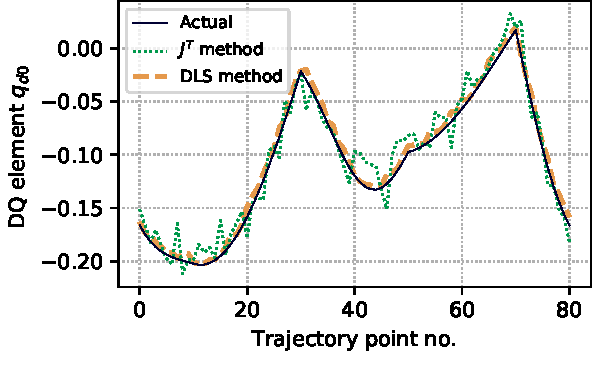
\includegraphics[width=0.4 \textwidth]{./imgs/trajectoryq4c.pdf}  }
%	\hfill
%	\subfloat{ 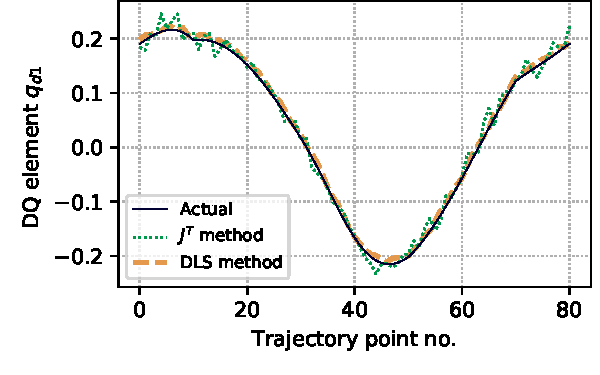
\includegraphics[width=0.4 \textwidth]{./imgs/trajectoryq5c.pdf}  }
%	\caption{ Comparison of DQ elements ($q_{d0}$ and $q_{d1}$) traced by $J^T$ and DLS IK models \cite{fernandez2015}}  \label{fig:dqelements}
%\end{figure}



%\begin{table}[h] \centering
%	\caption{ Frame transformations carried out using \cite{lentin2015} } \label{tab:screwmotions}
%	\begin {tabular}[h]	{| c | c  c |}	 \hline 
%	%	\begin {tabular}[h]	{| c | p{0.35\textwidth} | p{0.35\textwidth} |}	 \hline		
%	\shortstack{Frame \\ transformation}   &   $\left\lbrace i-1 \right\rbrace$ to $\left\lbrace i' \right\rbrace$   &   $\left\lbrace i' \right\rbrace$ to $\left\lbrace i \right\rbrace$ \\ \hline
%	Rotation angle $ \theta $   &   $ \theta_i $   &   $ \alpha_i $ \\ \hline
%	Rotation axis $ \hat{\vec{u}} $   &   $ ( 0, 0, 1 ) $   &   $ ( 1, 0, 0 ) $ \\ \hline
%	\shortstack{Translation \\ direction $ \vec{t} $ }  &   $ ( 0, 0, d_i ) $   &   $ ( a_i, 0, 0 ) $ \\ \hline
%	$ \hat{\vec{u}} \cdot \vec{t} $   &   $ d_i $   &   $ a_i $ \\ \hline
%	$ \hat{\vec{u}} \times \vec{t} $   &   $ 0 $   &    $ 0 $ \\ \hline
%	\shortstack{Transformation \\ DQ} & 
%	\shortstack {  $ \underline{q}^Z = \left[ C_\theta, \, 0, \, 0, \, S_\theta \right] +  \qquad $   \\   $ \qquad \epsilon \left[ -  D S_\theta, \, 0, \, 0, \, D C_\theta \right] $   }   &
%	\shortstack {  $ \underline{q}^X = \left[ C_\alpha, S_\alpha, 0, 0 \right] +  \qquad $   \\   $ \qquad \epsilon \left[ - A S_\alpha,  A C_\alpha, 0, 0 \right] $  }  \\ \hline \end{tabular} 
%\end{table}




\section{Summary of Jeroen Hol \cite{hol2008}}

Pose Estimation and Calibration Algorithms for Vision and Inertial Sensors \\  20088 \\  Division of Automatic Control \\  Department of Electrical Engineering \\  Link{\"o}ping University, Sweden

Augmented reality (AR) involves overlaying a real scene with computer generated graphics in real-time by showing the virtual objects on see-through head-mounted displays or superimposing them on live video imagery. In order to have realistic augmentation, i.e.,  positioning and aligning the virtual objects correctly with the real world, it is essential to know the position and orientation (pose) of the camera with high accuracy and low latency. A ?vision only approach? gives good absolute accuracy, but is difficult to run at high frame rate and is not robust during fast motions. An  inertial measurement unit (IMU) is accurate for a short period and is drift-prone for longer time scales. 

In this thesis, pose estimation is approached using a combination of a camera and an IMU. Using a 3D scene model containing natural landmarks removes the need for costly and time consuming procedure of preparing the environment, and allows for AR applications outside dedicated studios. The IMU unit provides rapid measurements of acceleration and angular velocity. The computer vision system generates correspondences between the camera image and a 3D scene model that contains positions of various natural markers and is generated offline using images and/or drawings of the scene. The camera pose is estimated by combining inertial and visual measurements in a sensor fusion model that solves a non-linear state estimation problem in real-time.

%Some aspects have been previously published in \\
%F. Gustafsson, T. B. Sch{\"o}n, and J. D. Hol. Sensor fusion for augmented reality. In Proceedings of 17th International Federation of Automatic Control World Congress, Seoul, South Korea, July 2008. Accepted for publication. \\
%J. D. Hol, T. B. Sch{\"o}n, H. Luinge, P. J. Slycke, and F. Gustafsson. Robust real-time tracking by fusing measurements from inertial and vision sensors. Journal of Real-Time Image Processing, 2(2):149?160, Nov. 2007. doi:10.1007/s11554-007-0040-2. \\
%J. D. Hol, T. B. Sch{\"o}n, F. Gustafsson, and P. J. Slycke. Sensor fusion for augmented reality. In Proceedings of 9th International Conference on Information Fusion, Florence, Italy, July 2006b. doi:10.1109/ICIF.2006.301604. \\
%J. D. Hol, T. B. Sch{\"o}n, and F. Gustafsson. On resampling algorithms for particle fil- ters. InProceedings of Nonlinear Statistical Signal Processing Workshop, Cambridge, UK, Sept. 2006a. doi:10.1109/NSSPW.2006.4378824. \\
%G. Hendeby, J. D. Hol, R. Karlsson, and F. Gustafsson. A graphics processing unit
%implementation of the particle filter. In Proceedings of European Signal Processing Conference, Pozn{\'a}n, Poland, Sept. 2007.

\subsection{Robust real-time tracking by fusing measurements from inertial and vision 	sensors} %	System overview

The pose of a camera is estimated in real-time by fusing measurements from inertial sensors (accelerometers and rate gyroscopes) and a camera. The non-linear state estimation is based on a multi-rate extended Kalman filter using a dynamic model with 22 states, where \SI{100}{\Hz} inertial measurements and \SI{12.5}{\Hz} correspondences from vision are processed.Vision measurements are based on natural landmarks, which are detected guided by pose predictions. The measurements from the sensors are used directly rather than being processed to a vision based pose or an inertial based pose. Accurate short time pose estimates are available using information from IMU hereby reducing the need for fast vision updates, which would otherwise require high frame rates and compute.

Coordinate systems used:
\begin{itemize}
	\item Earth $ e $: It is fixed to earth and generally vertically aligned.  The camera pose is estimated w.r.t. it and features of the scene are modeled in it.
	\item Camera $ c $: It is attached to the moving camera. Its origin is 	located in the optical center of the camera, with the $ z $-axis pointing along the optical axis. The camera acquires its images in the image plane $ (i) $. This plane is perpendicular to the optical axis.
	\item Body $ b $: It is the coordinate system of the IMU attached by a constant translation and rotation w.r.t. the camera.
\end{itemize}

These coordinate systems are used to denote geometric quantities, for instance, $ \bm{c}^e $ is the position of the camera coordinate system expressed in the earth system and $ R^{cb} $ is the rotation matrix from the body system to the camera system.

The IMU consists of \SI{1200}{\deg\per\s} gyroscopes and 5g accelerometers. The signals from the inertial components of the IMU are synchronously measured at \SI{100}{|\Hz} using a 16 bit A/D converter. A temperature sensor is added to compensate for the temperature dependency of the sensing components. The IMU sensor is subjected to a calibration procedure to calibrate for the exact physical alignment of each component, the gains, the offsets, and the temperature relations of the gains and offsets. With these, a 3D angular velocity vector and a 3D accelerometer vector, both resolved in the body coordinate system, are computed. The calibrated gyroscope signal $ \bm{y}_{\omega,t} $ contains measurements of the angular velocity $ \bm{\omega}^b_{eb,t} $ from body to earth $ ( _{eb} ) $ expressed in the body coordinate system $ ( ^b ) $:
\begin{equation}
\bm{y}_{\omega,t} = \bm{\omega}^b_{eb,t} + \bm{\delta}^b_{\omega,t} + \bm{e}^b_{\omega,t}
\end{equation}
Here, $ \bm{\delta}^b_{\omega,t} $ is the low-frequency offset fluctuations due toe unmodeled acceleration dependency and $ \bm{e}^b_{\omega,t} $ is zero mean white noise. A change in orientation is obtained by integration of the gyroscope signal without relying on any infrastructure. However, accuracy in orientation deteriorates for periods longer than a few seconds. 

The calibrated accelerometer signal $ \bm{y}_{a,t} $ contains measurements of the  combination of the body acceleration vector $ \ddot{\bm{b}}_{t} $ and the gravity vector $ \bm{g} $ both expressed in the body coordinate system $ ( ^b ) $:
\begin{equation}
\bm{y}_{a,t} = \ddot{\bm{b}}^b_{t} - \bm{g}^b_{t} + \bm{\delta}^b_{a,t} + \bm{e}^b_{a,t}
\end{equation}
Here, $ \bm{\delta}^b_{a,t} $ is the low-frequency offset and $ \bm{e}^b_{a,t} $ is zero mean white noise. Gravity expressed in body coordinates depends on the orientation of the sensor unit. Once the orientation is known, the accelerometer signal is used to estimate the acceleration, or alternatively, once the acc$\tpose[n]$ is known, the direction of the vertical is estimated. Acceleration is integrated twice to obtain change in position, as long as accurate orientation estimate is available from the gyroscopes. However, accuracy of position change deteriorates quickly as a result of double integration and orientation errors. 

The camera has a perspective lens with focal length of \SI{3.2}{\mm} and captures images with a resolution of $ 320 \times 240 $ pixels at a frame-rate of \SI{12.5}{Hz}.  The camera is triggered by the IMU clock allowing for synchronized measurements. Extracting camera position and orientation from images is a known and well studied problem in computer vision. The key ingredient is to find correspondences, i.e., relations between features in the image which correspond to an element in the scene model. Point correspondences $ \bm{z}^{c} \leftrightarrow \bm{z}^{i} $ are the relation between 3D points $ \bm{z}^{c} $ and 2D image points $ \bm{z}^{i} $.  For a perspective lens and a pinhole camera, the correspondence relation is

\begin{subequations}
	\begin{equation}
	\bm{z}^{i} = \Bmtrx{f z_{c}^{x} / z_{c}^{z} \\ f z_{c}^{y} / z_{c}^{z} } + \bm{e}^{i} \newline
	\end{equation}
	\text{or equivalently,}
	\begin{equation}
	\bm{0} \approx \Bmtrx{ -f\bm{I}_{2} & \bm{z}_{t}^{i} } \bm{z}_{t}^{c} = \Bmtrx{ -f\bm{I}_{2} & \bm{z}_{t}^{i} } \bm{R}_{t}^{cc} \left( \bm{z}^{c} - \bm{z}_{t}^{c} \right) 
	\end{equation}
\end{subequations}
where $ f $ is the focal length, $ \bm{I}_{2} $ is $ 2 \times 2 $ identity matrix, $ \bm{e}_{t}^{i} $ is zero-mean white noise. The camera pose depends on the rotation matrix $ R^{ce} $ and the position $ \bm{c}^{c} $. Hence, given sufficient  correspondences and a calibrated camera, the camera pose can be found. 

The computer vision implementation is based on a sum of absolute difference (SAD) block matcher in combination with a planar patch or free-form surface model of the scene. Both pixel data and 3D positions are stored for each feature. While tracking, search templates are generated by warping the patches in the model according to homographies calculated from the latest prediction of the camera pose. These templates are then matched with the current calibrated camera image using the block matcher. In this way correspondences are generated.


\subsubsection{Sensor fusion}

Vision in combination with the map gives accurate absolute pose information at a low rate, but experiences problems during moderately fast motions. The IMU provides high rate relative pose information regardless of the motion speed, but becomes inaccurate after a short period of time. By fusing information from both sources, it is possible to obtain robust camera pose estimates.

One way is to extend vision-based methods by using pose predictions from the IMU to determine where in the image the features are to be expected. Once detected, the features are used to calculate the pose, and this pose is then used as a starting point for the next pose prediction by the IMU. Another way is to consider IMU to be the main sensor, which is quite common in the navigation industry. Then vision is used for error correction, similar to how radio beacons or global positioning system (GPS) are used to correct the drift in an inertial navigation system (INS). 

The objective in filtering is to extract as much information as possible from the measurements. More specifically, this amounts to finding the best possible estimate of the filtering probability density function (pdf) $ p( x_{t} | y_{1:t} ) $ where $ y_{1:t} \triangleq %\overset{\Delta}{=}
\{ y_{1}, \ldots, y_{t} \} $. The objective in sensor fusion is to recursively in time estimate the state in the dynamic model,
\begin{subequations} \label{eq:fusion} \begin{align}
	x_{t+1} &= f_{t} ( x_{t} ,u_{t} , v_{t} )\\
	y_{t} &= h_{t} ( x_{t} ,u_{t} , e_{t} )
\end{align} \end{subequations}
where $ x_{t} \in \mathbb{R}^{n_{x}} $ denotes state estimate, $ y_{t} \in \mathbb{R}^{n_{y}} $ denotes  measurements from sensors, $ v_{t} $ and $ e_{t} $ denote the stochastic process and measurement noise respectively, $ f : \mathbb{R}^{n_{x}} \times \mathbb{R}^{n_{u}} \times \mathbb{R}^{n_{v}} \rightarrow \mathbb{R}^{n_{x}} $ is process model that describes evolution of state over time, and $ h : \mathbb{R}^{n_{x}} \times \mathbb{R}^{n_{u}} \times \mathbb{R}^{n_{e}} \rightarrow \mathbb{R}^{n_{y}} $ is measurement model that describes how measurements from IMU and  camera relate to the state.  

The goal is to infer information from measurements $ y_{t} $ onto the state $ x_{t} $ by computing the filtering pdf $ p ( x_{t} | y_{1:t} ) $.  The filtering pdf contains everything there is to know about the state at time $ t $, given the information in all the past measurements $ y_{1:t} $. The approximation of $ p ( x_{t} | y_{1:t} ) $ is used to form different (point) estimates, including maximum likelihood estimates, confidence intervals and expectation estimate $ \hat{x}_{t} = E( x_{t} | y_{1:t} ) $. The key element in solving the nonlinear state estimation problem in real-time is the propagation of $ p ( x_{t} | y_{1:t} ) $ over time. 

\begin{subequations}\label{eq:update1} \begin{align}
	p ( x_{t} | y_{1:t} ) &= \frac { p ( y_{t} | x_{t} ) p ( x_{t} | y_{1:t-1} ) } { \int p ( y_{t} | x_{t} ) p ( x_{t} | y_{1:t-1} ) \dd{x_{t}} } \label{subeq:measupd1}\\
	p ( x_{t+1} | y_{1:t} ) &= \int p ( x_{t+1} | x_{t} ) p ( x_{t} | y_{1:t} ) \dd{x_{t}} \label{subeq:timeupd1}
\end{align} \end{subequations}

Eqs. \ref{subeq:measupd1} and \ref{subeq:timeupd1}  are called measurement update and time update, respectively.  The sensor fusion problem is reduced to propagating eq. \ref{eq:update1} over time as new measurements arrive. When eq. \ref{eq:fusion} is linear and noise is Gaussian, then involved densities become Gaussian and updating recursions are given by the Kalman Filter (KF). It is sufficient to assume that noise enters additively, according to
\begin{subequations} \begin{align}
	x_{t+1} &= f_{t} ( x_{t} ) + v_{t} \\
	y_{t} &= h_{t} ( x_{t} ) + e_{t}
\end{align} \end{subequations}

Additive noise modifies Eq. \ref{eq:update1} to
\begin{subequations} \begin{align}
	p ( x_{t+1} | x_{t} ) &= p_{v_{t}} ( x_{t+1} - f_{t} ( x_{t} ) ) \\
	p ( y_{t} | x_{t} ) &= p_{e_{t}} ( y_{t} - h_{t} ( x_{t} ) )
\end{align} \end{subequations}
where $ p_{v_{t}} (\cdot) $ and $ p_{e_{t}} (\cdot) $ denote the pdf's for the noise $ v_{t} $ and $ e_{t} $, respectively.

The state vector consists of position of the IMU (the body coordinate system) expressed in the earth system $ b^{e} $, its velocity $ \dot{\bm{b}}^{e} $ and acceleration $ \ddot{\bm{b}}^{e} $, the orientation (quaternion) of the body wrt earth $ q^{be} $, its angular velocity $ \omega_{eb}^{b} $, the gyroscope bias $ \delta_{\omega}^{b} $ and the accelerometer bias $ \delta_{a}^{b} $. The state vector has dimension 22 and is given by
\begin{equation}\label{eq:state1}
x_{t} = \Bmtrx{ \bm{b}_{t}^{e} \\ \dot{\bm{b}}_{t}^{e} \\ \ddot{\bm{b}}_{t}^{e} \\ q_{t}^{be} \\ \bm{\omega}_{eb,t}^{b} \\ \bm{\delta}_{\omega,t}^{b} \\ \bm{\delta}_{a,t}^{b} }
\end{equation}

The process model is given by
\begin{subequations}\label{eq:procmod1} \begin{align}
	\bm{b}_{t+1}^{e} &= \bm{b}_{t}^{e} + T \dot{\bm{b}}_{t}^{e} + \tfrac {T^{2}} {2} \ddot{\bm{b}}_{t}^{e} \\
	\dot{\bm{b}}_{t+1}^{e} &= \dot{\bm{b}}_{t}^{e} + T \ddot{\bm{b}}_{t}^{e} \\
	\ddot{\bm{b}}_{t+1}^{e} &= \ddot{\bm{b}}_{t}^{e} + \bm{v}_{b,t}^{e} \\
	q_{t+1}^{be} &= \exp( -\tfrac{T}{2} \bm{\omega}_{eb,t}^{b} ) \odot q_{t}^{be} \\
	\bm{\omega}_{eb,t+1}^{b} &= \bm{\omega}_{eb,t}^{b} + \bm{v}_{\omega,t}^{b} \\
	\bm{\delta}_{\omega,t+1}^{b} &= \bm{\delta}_{\omega,t}^{b} + \bm{v}_{\delta_{\omega},t}^{b} \\
	\bm{\delta}_{a,t+1}^{b} &= \bm{\delta}_{a,t}^{b} + \bm{v}_{\delta_{a},t}^{b}
\end{align} \end{subequations}
where the quaternion multiplication and exponential are defined according to
\begin{subequations} \begin{align}
	\Bmtrx{ p_{0} \\ \bm{p} } \odot \Bmtrx{ q_{0} \\ \bm{q} } &\triangleq \Bmtrx{ q_{0} q_{0} - \bm{p} \cdot \bm{q} \\ q_{0} \bm{q} + q_{0} \bm{p} + \bm{p} \times \bm{q} } \\
	\exp( \bm{v} ) &\triangleq \Bmtrx{ \cos \| \bm{v} \| \\ \tfrac { \bm{v} }{ \| \bm{v} \| } \sin \| \bm{v} \| }
\end{align} \end{subequations}

The measurement models are given by
\begin{subequations} \label{eq:measmod1} \begin{align}
	\bm{y}_{a,t} &= R_{t}^{be} ( \ddot{\bm{b}}_{t}^{e} - \bm{g}^{e} ) + \bm{\delta}_{a,t}^{b} + \bm{e}_{a,t}^{b} \label{subeq:accel}\\
	\bm{y}_{\omega,t} &= \bm{\omega}_{eb,t}^{b} + \bm{\delta}_{\omega,t}^{b} + \bm{e}_{\omega,t}^{b} \label{subeq:gyro}\\
	\bm{y}_{c,t} &= \Bmtrx{ -f\bm{I}_{2} & \bm{z}_{t}^{i} } \bm{R}^{cb} ( \bm{R}_{t}^{be} ( \bm{z}_{t}^{e} - \bm{b}_{t}^{e} ) - \bm{c}^{b} )  + \bm{e}_{a,t}^{b} \label{subeq:cam}
\end{align} \end{subequations}
The rotation matrix $ \bm{R}_{t}^{be} $ is constructed from $ q_{t}^{be} $. The transformation from body to camera coordinate system is included in vision measurement.

Algorithm \ref{alg:orient-ekf1} uses models in Eqs. \ref{eq:procmod1} and \ref{eq:measmod1} to perform updates given in Eq. \ref{eq:update1}. The algorithm runs in real time with inertial measurements at \SI{100}{Hz} and frame rates up to \SI{25}{Hz} and uses EKF to compute pose estimates. 

%\hrulefill \vspace{-0.5\baselineskip} \captionof{algorithm}{Recursive camera pose calculation}\label{alg:orient-ekf1}  \hrule
%%\begin{algorithm}
%%	\caption{Orientation estimation using EKF with orientation deviation states \cite{kok2017} }  \label{alg:dq-pose-err1}
%\begin{algorithmic}[1]
%	\INPUT Inertial data $ \lbrace \bm{y} _{a,t} , \bm{y} _{\omega,t}  \rbrace _{t=1} ^{N} $, magnetometer data $ \lbrace \bm{y} _{m,t}  \rbrace _{t=1} ^{N} $ 
%	\OUTPUT  Orientation estimate  and covariance $ \bm{P} _{t | t} $ for $ t = 1, \cdots, N $
%	\FOR { $ t = 2 $ \TO $ N $ }     
%		\STATE Time update. Calculate $ p( \bm{x}_{t} | \bm{y}_{1:t-1} ) $ by propagating $ p( \bm{x}_{t-1} | \bm{y}_{1:t-1} ) $ through process model Eq. \ref{eq:proc1}.
%%		\STATE \COMMENT{\textbf{Measurement update:}}
%		\STATE Accelerometer and gyroscope measurement update using model Eqs. \ref{subeq:accel} and \ref{subeq:gyro}.
%		\STATE $ \qquad\qquad \bm{x}_{t} \sim p ( \bm{x}_{t} | \bm{y}_{1:t} ) $
%		\IF {there is a new image from the camera}
%			\STATE  Predict feature positions from the scene model using $ \hat{\bm{x}}_{t} = E( \bm{x}_{t} | \bm{y}_{1:t} ) $.
%			\STATE Detect features in the image.
%			\STATE  Measurement update with the found point correspondences using model Eq. \ref{subeq:cam}.
%			\STATE $ \qquad\qquad \bm{x}_{t} \sim p ( \bm{x}_{t} | \bm{y}_{1:t} ) $
%		\ENDIF
%	\ENDFOR
%\end{algorithmic} \vspace{-0.75\baselineskip} \hrulefill
%%\end{algorithm}

\begin{algorithm}[H]
	\caption{Recursive camera pose calculation}\label{alg:orient-ekf1}
	\DontPrintSemicolon \SetAlgoLongEnd \SetAlgoLined 
	\SetKwInOut{Output}{Output} \SetKwInOut{Input}{Input}
	\Input{Inertial data $ \lbrace \bm{y} _{a,t} , \bm{y} _{\omega,t}  \rbrace _{t=0} ^{N} $\\ Magnetometer data $ \lbrace \bm{y} _{m,t}  \rbrace _{t=0} ^{N} $ \; } 
	\Output{Pose estimate  $ \bm{x} _{t} $ for $ t = 1, \cdots, N $ \; }
	\For{ $ t = 1 $ \KwTo $ N $ } {    % \tcp{Time update:}
		Time update. Calculate $ p( \bm{x}_{t} | \bm{y}_{1:t-1} ) $ by propagating $ p( \bm{x}_{t-1} | \bm{y}_{1:t-1} ) $ through process model Eq. \ref{eq:procmod1}. \;
		Accelerometer and gyroscope measurement update using model Eqs. \ref{subeq:accel} and \ref{subeq:gyro}. \;
       	$ \qquad\qquad \bm{x}_{t} \sim p ( \bm{x}_{t} | \bm{y}_{1:t} ) $ \;
		\If{there is a new image from the camera}{
			Predict feature positions from the scene model using $ \hat{\bm{x}}_{t} = E( \bm{x}_{t} | \bm{y}_{1:t} ) $. \;
			Detect features in the image. \;
			Measurement update with the found point correspondences using model Eq. \ref{subeq:cam}. \;
			$ \qquad\qquad \bm{x}_{t} \sim p ( \bm{x}_{t} | \bm{y}_{1:t} ) $ \;
		} % end if
	} % end for
\end{algorithm}

The camera and the IMU both deliver measurements which are resolved respectively in the camera and the body coordinate system. As the sensors are physically translated and rotated with respect to each other, this rigid transformation should be taken into account while fusing the measurements.  

The high frequency inertial measurement updates provide a rather accurate state estimate when a new image is acquired. This implies that the feature positions can be predicted with an improved accuracy, which in turn makes it possible to use a guided search in the image using reduced search regions. The algorithm can calculate the expected covariance of a measurement. 

The information from the IMU makes Algorithm \ref{alg:orient-ekf1} robust for temporary absence of vision due to motion blur, obstruction of the camera or unmodeled scene. Without vision measurements, the estimates will eventually drift away. The algorithm is flexible and can be rather straightforwardly extended to include other information sources. When the sensor unit is static during initialization, the IMU provides partial or full orientation estimates (using magnetometers). This information is used to constrain the search space when initializing from vision.

Vision-only methods suffer from scale ambiguity, since projections are used. Changing the scale of a scene model will give scaled, but indistinguishable poses. As sensor fusion utilizes position information both from the camera and the IMU, the scale is relevant and these quantities must have identical units. Introducing a metric scale into the scene model solves this issue. An existing scene model with arbitrary scale can be converted by comparing it with a CAD model or by measuring an object with known dimension.

To separate the contribution of gravity in acceleration measurement, the gravity vector is rotated from earth frame to body frame and subtracted. The scene model should be vertically aligned, or the gravity vector should be known in the scene model. But, this is not the case. The performance of the system is extremely sensitive to this alignment, since gravity is typically an order of magnitude larger than normal body accelerations. A misalignment of \ang{1} introduces an artificial acceleration of \SI{0.17}{\m\per\s\squared} which gives rise to a systematic position drift of \SI{8.5}{\cm} when integrated over \SI{1}{\s}. Hence, even for small errors, a systematic drift is introduced which causes the system to lose track without continuous corrections from correspondences. Drifts followed by a correction gives rise to a saw tooth pattern in the estimates, which is visible as `jitter'. The gravity vector can be determined by averaging the accelerometer readings over some time, while the camera is stationary in a known pose. However, a preferable method is to record accelerometer measurements while scanning the scene and include this data in the model building procedure to align the scene model vertically.


\subsubsection{Implementation considerations}  

\textbf{Sensor pose calibration}: The problem of determining the relative position and orientation is a well studied problem in robotics where it is known as hand-eye calibration. However, most methods do not apply directly since the IMU does not provide an absolute position reference. Absolute orientation is available when the IMU is stationary, since the accelerometers measure only gravity. The orientation part of the calibration is determined using a slight modification of standard camera calibration procedures. As floors and desks in buildings are better horizontally aligned than walls are vertically aligned, it is recommended to use horizontal surfaces. The calibration pattern is placed on a horizontal surface and accelerometer readings are taken at various camera poses. The camera poses are determined in the camera calibration procedure, from which the vertical directions in the camera frame are determined. The combination of these and the vertical directions in the body frame measured by the accelerometers allows for calculation of the rotation between the frames. This method requires accurate positioning of the calibration pattern. 

\textbf{Time synchronization}: It is very important to know exactly when the different measurements are taken. Time synchronization between clocks of multiple sensors is achieved by hardware synchronization, i.e., one central clock is used to trigger the other sensors. This solves the problem of simultaneously started clocks diverging after operating for a while. 

\textbf{Filter tuning}: The models have stochastic components which are used to tune the EKF (Refer Table 2.1 in report page 21). For IMU, noise covariance is calculated either experimentally from measurements of a few seconds with a static pose, or directly from manufacturer specification. The noise in vision measurements is harder to determine as accuracy for each match is highly individual, and variations due to lighting conditions, local texture, viewing angle, distance and motion blur cannot be captured by a common noise setting. Hence, it would be beneficial to include accuracy estimation in the image processing algorithms. 
The current implementation uses a predefined noise covariance. Again, the process model is a random walk in acceleration and angular velocity, and though not informative, the model is useful for tracking uncontrolled motions such as those generated by a human. Also, the motion model is to be considered as a separate source of information, apart from the sensors. Including additional information (such as control signals) in the model improves filter performance. The covariances in the process model can be seen as tuning knobs, controlling the relative importance of the measurements and the process model and as such they are important parameters for stable tracking. The innovations, defined as the difference between a measurement and its expected value, $ e_{t} = y_{t} - \hat{y_{t}} $, asses whether the models are correctly tuned. The innovations should be normally distributed, and the squared normalized innovations $ e_{t}\tpose {S_{t}}\tpose[-1] e^{t} $, where $ S_{t} $ is the predicted covariance of the measurement, should have a $ \chi^{2} $ distribution. These performance indicators should be monitored during both testing and normal operation.

\subsubsection{Experiments}

The sensor unit is mounted onto a 6 degrees of freedom (DoF) ABB IRB1440 industrial robot. The robot allows repeatable 6 DoF motions, provides true positions and orientations, and has an absolute accuracy of \SI{2}{\mm} and repeatability of \SI{0.2}{\mm}. This enables systematic and objective performance evaluation of algorithms based on absolute pose errors, instead of the usual feature reprojection errors. The scene used for experiments consists of two orthogonal planar surfaces constructed from a textured CAD model. It's x-axis points upward, y and z-axes span the horizontal plane, and has to be calibrated w.r.t. gravity. The sensor unit traverses a \SI{2.6}{\m} eight-shaped trajectory in \SI{5.4}{\s}, keeping the scene in view at all times. The motion contains accelerations up to \SI{4}{\m\per\s\squared} and angular velocities up to \SI{1}{\radian\per\s}. As the displacement between images is limited to 15 pixels it is still possible to use vision-only tracking, which allows for a comparison between tracking with and without an IMU. The experiment starts with a synchronization motion to synchronize the ground truth data from the industrial robot with the estimates from the system. Time synchronization is relevant, since a small time offset between the signals will result in a significant error. After the synchronization, the eight-shaped trajectory is repeated several times, utilizing the accurate and repeatable motion provided by the industrial robot.




%\[ \pdv{f}{x}{y}  \pdv[3]{f}{t}  \pdv*[3]{f}{x} \pdv[3]{t} \]















\section{Reviews}

%\begin{landscape}
%	After this point, everything is displayed in landscape format.\\
%\pagebreak
\begin{longtable}[c]{|p{0.25\textwidth}|p{0.13\textwidth}|p{0.30\textwidth}|p{0.2\textwidth}|} 
	%\hline\hline \multicolumn{4}{| c |}{\textit{Begin of Notes}}\\ 
	%\endfirsthead
	\hline 	\textbf{ID, Title, Author, Journal} 	&  \textbf{Research areas, Tools}  &  \textbf{Objectives, Methodology, Discussion}  &  \textbf{Conclusions, My inference, Gaps} \\ \endhead
	%\hline \endfoot
	\hline\multicolumn{4}{| c |}{\textit{End of Notes}}\\ \hline\hline \endlastfoot
	% ---------------------------------------------------------
	\hline  \multiline { \item\textbf{authyear}    \item\textit{paper title}    \item firstname1 surname1 and firstname2 surname2    \item journal } 
	&  \multiline{ \item keyword1    \item keyword2 }
	&  \multiline{ \item objec    \item method    \item concl } 
	&  \multiline {\item gap } \\
	% ---------------------------------------------------------
	\hline  \multiline { \item\textbf{aydin2006}    \item\textit{Quaternion Based Inverse Kinematics for Industrial Robot Manipulators with Euler Wrist}    \item Yavuz Ayd{\i}n and Serdar Kucuk    \item IEEE 3rd International Conference on Mechatronics (ICM 2006) } 
	&  \multiline{ \item wrist IK    \item quaternion-vector pair for 6-dof pose }
	&  \multiline{ \item Double quaternion instead of dual quaternion    \item Approximate translation magnitue $d$ as rotation by angle $\psi = \dfrac{d}{R}$ about normalised vector $d$. } 
	&  \multiline {\item Results obtained by using double quaternions are coordinate frame invariant. } \\
	% ---------------------------------------------------------
	\hline  \multiline { \item\textbf{ge1998} \item\textit{Double quaternions for motion interpolation} \item Ge, Q J and Varshney, Amitabh and Menon, Jai P and Chang, Chu-Fei \item --- } 
	&  \multiline{ \item dual quaternions }
	&  \multiline{ \item Double quaternion instead of dual quaternion \item Approximate translation magnitue $d$ as rotation by angle $\psi = \dfrac{d}{R}$ about normalised vector $d$. } 
	&  \multiline {\item Results obtained by using double quaternions are coordinate frame invariant. } \\
	% ---------------------------------------------------------
	\hline  \multiline { \item\textbf{authyear}    \item\textit{paper title}    \item firstname1 surname1 and firstname2 surname2    \item journal } 
	&  \multiline{ \item keyword1    \item keyword2 }
	&  \multiline{ \item objec    \item method    \item concl } 
	&  \multiline {\item gap } \\
	% ---------------------------------------------------------
	\hline  \multiline { \item\textbf{authyear}    \item\textit{paper title}    \item firstname1 surname1 and firstname2 surname2    \item journal } 
	&  \multiline{ \item keyword1    \item keyword2 }
	&  \multiline{ \item objec    \item method    \item concl } 
	&  \multiline {\item gap } \\
	% ---------------------------------------------------------
	\hline  \multiline { \item\textbf{ge1998} \item\textit{Double quaternions for motion interpolation} \item Ge, Q J and Varshney, Amitabh and Menon, Jai P and Chang, Chu-Fei \item --- } 
	&  \multiline{ \item dual quaternions }
	&  \multiline{ \item Double quaternion instead of dual quaternion \item Approximate translation magnitue $d$ as rotation by angle $\psi = \dfrac{d}{R}$ about normalised vector $d$. } 
	&  \multiline {\item Results obtained by using double quaternions are coordinate frame invariant. } \\
	% ---------------------------------------------------------
	\hline \multiline{\item\textbf{thomas} \item\textit{Approaching Dual Quaternions from Matrix Algebra} \item Frederico Thomas \item --- }
	&\multiline{\item double quaternion derivation}
	&
	& \\
	% ---------------------------------------------------------
	
\end{longtable}
%\end{landscape}
%After this point, everything is displayed in portrait format.\\









\bibliographystyle{unsrt}
\bibliography{mybibliography} 

\end{document}